\documentclass{article} % For LaTeX2e
\usepackage{iclr2027_conference,times}
% Optional math commands from https://github.com/goodfeli/dlbook_notation.
\input{math_commands.tex}
\usepackage{hyperref}
\hypersetup{hypertexnames=false}
\usepackage{url}
\usepackage{booktabs}
\usepackage{graphicx}
\usepackage{multirow}
\usepackage{amsmath}
\usepackage{amssymb}
\usepackage{colortbl}
\usepackage{xcolor}
\usepackage{enumitem}
\usepackage{float}
\usepackage{algorithm}
\usepackage[noend]{algpseudocode}
\usepackage{wrapfig}
\usepackage{capt-of}
\setlength{\textfloatsep}{10pt plus 2pt minus 2pt}
\setlength{\intextsep}{10pt plus 2pt minus 2pt}
\setlength{\abovecaptionskip}{5pt}
\setlength{\belowcaptionskip}{0pt}
\title{OpenAgency: Self-Evolving Multi-Agent System via Governed Collaboration Protocols}
% Authors must not appear in the submitted version. They should be hidden
% as long as the \iclrfinalcopy macro remains commented out below.
% Non-anonymous submissions will be rejected without review.
\author{Anonymous authors}
% The \author macro works with any number of authors. There are two commands
% used to separate the names and addresses of multiple authors: \And and \AND.
%
% Using \And between authors leaves it to \LaTeX{} to determine where to break
% the lines. Using \AND forces a linebreak at that point. So, if \LaTeX{}
% puts 3 of 4 authors names on the first line, and the last on the second
% line, use \AND before the third author name when a forced line break is needed.
\newcommand{\fix}{\marginpar{FIX}}
\newcommand{\new}{\marginpar{NEW}}
%\iclrfinalcopy % Uncomment for camera-ready version, but NOT for submission.
\begin{document}
\maketitle

\begin{abstract}
Large language model (LLM) agents have demonstrated strong capabilities in solving complex tasks, motivating the development of multi-agent systems (MAS) that coordinate agents with specialized roles. However, existing multi-agent collaboration paradigms are often static, with collaboration patterns determined a priori and remaining unchanged during execution. Enabling continuously improving collaboration requires protocols that balance flexibility and controllability: flexibility allows agents to explore diverse coordination strategies at runtime, while controllability ensures that such decisions can be used to improve collaboration.
Existing collaboration protocols typically fall into two extremes: they are either rigidly predefined, limiting adaptation, or fully free-form, sacrificing oversight. In this paper, we introduce OpenAgency, a self-evolving multi-agent system built upon governed collaboration protocols. These protocols enable agents to dynamically select their next collaborators within a predefined yet extensible space at runtime, transforming the collaboration pattern itself into an evolvable object.
To evolve collaboration protocols, OpenAgency maintains execution traces from agent interactions and introduces a collaboration-driven evolving agent that distills these experiences into a bounded number of atomic protocol improvements. Through this mechanism, OpenAgency allows multi-agent systems to continuously refine their collaboration strategies and adapt to diverse complex tasks while preserving control over the evolution process.
Experiments across fourteen benchmarks spanning general question answering, long-horizon reasoning tasks, and production-oriented workloads demonstrate that OpenAgency achieves improved collaboration performance and continues to enhance its effectiveness through self-evolution.\footnote{Code is available in the supplementary material.}
\end{abstract}

\section{Introduction}

% Large language models (LLMs)~\citep{gpt4,chatgpt} have shown strong capabilities on complex tasks such as software engineering~\citep{yang2024sweagent,wang2024openhands,zhang2024autocoderover}, data research~\citep{liu2026ddrbench,li2024deveval}, and long-horizon planning~\citep{zhang2026deepplanning,xu2024theagentcompany}. Multi-agent systems built on LLMs extend these capabilities by assigning complementary roles that exchange intermediate evidence~\citep{wang2024survey,xi2023rise,hong2024metagptmetaprogrammingmultiagent,qian2024chatdevcommunicativeagentssoftware,wu2023autogenenablingnextgenllm}, which lets one system plan and verify the same task through cooperation. However, as tasks become longer and more heterogeneous, the collaboration process itself becomes both a source of errors and an underused source of improvement.

% Evolving the way agents collaborate requires flexibility and controllability at the same time. Flexibility matters because a multi-agent system has to recover what went wrong across roles, and one that cannot repair a failed handoff at runtime loses the remainder of the run with it. Controllability is equally necessary, since an update is informative only when the system can tell which coordination step was responsible and can verify that the revised collaboration remains admissible. Once either property is missing, cross-run improvement falls back to a blind search driven by the final score. For instance, on SWE-bench Verified~\citep{jimenez2024swebench}, a free-form multi-agent baseline reaches only $51.4\%$ file match and a standard operating procedure (SOP) baseline reaches $59.8\%$, far below the $86.2\%$ attained once the collaboration itself can be revised from execution traces (Table~\ref{tab:free_form}).

% Existing collaboration representations hold only one of these two properties. \emph{Blueprint-driven} systems encode a graph, workflow, or standard operating procedure~\citep{hong2024metagptmetaprogrammingmultiagent,wu2023autogenenablingnextgenllm,fourney2024magenticonegeneralistmultiagentsolving}, and recent methods automate this design through workflow search or generated agent programs~\citep{zhang2025aflowautomatingagenticworkflow,hu2025automateddesignagenticsystems,zhang2025maasagenticsupernet}. Such designs are controllable, yet each selected workflow still determines the exact route taken during execution, and a runtime deviation therefore cannot be repaired locally. \emph{Agent-driven} systems let debate, dialogue, or dynamic connectivity emerge at runtime~\citep{li2023camelcommunicativeagentsmind,du2023improvingfactualityreasoninglanguage,liu2024dynamicllmpoweredagentnetwork,park2023generativeagentsinteractivesimulacra}, and a learned orchestrator can further reorder agent activations from reward~\citep{dang2025puppeteer}. Flexibility here costs transparency, since the realized coordination stays opaque and is hard to attribute or revise across runs. One line of work fixes the route and the other hides it, so neither yields a representation that is checkable at runtime and revisable from experience.

% In this paper, we aim to make the collaboration pattern itself evolvable by holding flexibility and controllability in one representation. To this end, we introduce \emph{OpenAgency}, a self-evolving multi-agent system built on \emph{governed collaboration protocols}. As illustrated in Figure~\ref{fig:intro}, OpenAgency represents a protocol as a tuple $\mathcal{P}=(\mathcal{R},\mathcal{N},\alpha,\mathcal{H},\mu,\Omega,\mathcal{C})$ whose components fix the roles and the admissible handoffs between them. The admissible handoff set $\Gamma(n,s)$ carries both properties in a single object, since it rules out inadmissible transitions while the choice inside it is left to the agent at runtime. Because every coordination decision is expressed in this object and its legality is decidable, the collaboration pattern becomes revisable between runs. Building on this, OpenAgency records accepted handoffs, rejected handoffs, completion events, and failures in a trace, and a collaboration-driven evolving agent turns this evidence into at most $k$ atomic edits over the protocol. A validity operator $\Pi_{\mathcal{V}}$ filters malformed topologies and the same agent scores the coordination each surviving candidate realizes, so every deployed round stays admissible and traceable to the events that motivated it.

% Experiments across fourteen benchmarks covering general question answering, long-horizon tasks, and production-oriented tasks show that OpenAgency achieves the best primary metric on every benchmark, lifting the unstructured multi-agent initialization by $20.7$ absolute points on average (Table~\ref{tab:main}). To the best of our knowledge, OpenAgency is the first multi-agent system in which the collaboration pattern is an evolvable object, updated from execution traces without regenerating the whole workflow. We summarize our contributions as follows.


Large language models (LLMs)~\citep{chatgpt} have shown strong capabilities on increasingly complex tasks, including software engineering~\citep{yang2024sweagent,wang2024openhands,zhang2024autocoderover}, data research~\citep{liu2026ddrbench,li2024deveval}, and long-horizon planning~\citep{zhang2026deepplanning,xu2024theagentcompany}. Building upon these capabilities, LLM-based multi-agent systems further improve task-solving ability by assigning agents complementary roles and enabling them to exchange intermediate information through communication~\citep{wang2024survey,xi2023rise,hong2024metagptmetaprogrammingmultiagent,qian2024chatdevcommunicativeagentssoftware,wu2023autogenenablingnextgenllm}. However, as tasks become longer, more diverse, and increasingly open-ended, the collaboration process itself becomes a new source of failure, since ineffective coordination, unnecessary interactions, and inappropriate delegation accumulate errors throughout execution. A multi-agent system therefore has to keep improving the way its agents collaborate, and not only the way each agent reasons.

However, evolving collaboration is non-trivial as it asks for two properties that pull against each other. Flexibility lets a system explore different coordination patterns and compare what they produce, which is how a better way to cooperate is found. Controllability lets the system identify which coordination decision contributed to success or failure and verify that a revised collaboration remains valid. Without flexibility, evolution degenerates into selecting among a fixed set of predefined strategies. Without controllability, improvement becomes blind optimization guided only by final task rewards, with little account of how or why a collaboration pattern changes.

Existing collaboration protocols typically provide only one of these properties, which limits how far they can be evolved. \emph{Blueprint-driven} approaches encode collaboration as graphs, workflows, or standard operating procedures~\citep{hong2024metagptmetaprogrammingmultiagent,wu2023autogenenablingnextgenllm,fourney2024magenticonegeneralistmultiagentsolving}, and later work automates such designs through workflow search or generated agent programs~\citep{zhang2025aflowautomatingagenticworkflow,hu2025automateddesignagenticsystems,zhang2025maasagenticsupernet}. Because the coordination structure is written down, these approaches are controllable, yet once a workflow is instantiated the execution follows a predetermined route and the collaboration cannot be adapted locally when an unexpected situation arises. \emph{Agent-driven} approaches let communication patterns, debates, or agent connectivity emerge at runtime~\citep{li2023camelcommunicativeagentsmind,du2023improvingfactualityreasoninglanguage,liu2024dynamicllmpoweredagentnetwork,park2023generativeagentsinteractivesimulacra}, and learned orchestrators adjust agent activation orders from feedback~\citep{dang2025puppeteer}. These approaches are flexible, yet the coordination they realize stays implicit and hard to attribute or revise across runs. In essence, neither line offers a collaboration protocol that is adaptable during execution and revisable afterwards.

In this paper, we make the collaboration protocol itself carry both properties, so that the collaboration pattern becomes an evolvable object. To this end, we introduce \emph{OpenAgency}, a self-evolving multi-agent system built upon \emph{governed collaboration protocols}. As illustrated in Figure~\ref{fig:intro}, a protocol specifies the agent roles and the handoffs admitted between them, fixing a set of valid coordination choices without committing to one execution path. An agent selects its next collaborator at runtime from inside that set, which supplies the flexibility, while the set rules out every transition the protocol does not admit, which supplies the controllability. Both properties therefore live in the same protocol, where each transition is checkable before it is taken and the collaboration pattern becomes something a later run can inspect and revise.
On top of this protocol, OpenAgency adds an evolution loop that keeps improving the deployed collaboration. Each run leaves a trace that records accepted handoffs, rejected handoffs, completion events, and failures, so the coordination evidence prior systems discard stays available afterwards. A collaboration-driven evolving agent reads that trace and proposes at most four atomic edits over the protocol. A validity operator filters malformed topologies and the same agent scores the coordination each surviving candidate realizes, so every deployed round stays admissible and traceable to the events that motivated it. To the best of our knowledge, OpenAgency is the first multi-agent system that treats the collaboration pattern itself as an evolvable object, improving it from execution traces while runtime validity and interpretability are preserved. We summarize our contributions as follows.
\begin{itemize}[leftmargin=1em, itemsep=0ex, topsep=0ex]
    \item \textbf{Evolvable Collaboration Protocol:} We make the collaboration pattern itself a governed and evolvable object, because the admissible handoff set is checkable before a transition is taken and revisable after the run that produced it.
    \item \textbf{Collaboration-driven Evolution:} We propose an evolving agent that learns from the coordination evidence prior systems discard. A validity operator and a collaboration quality check keep every deployed round admissible and free of regression.
    \item \textbf{Strong Performance:} Experiments across fourteen benchmarks spanning general question answering, long-horizon reasoning, and production-oriented tasks show that OpenAgency reaches the best primary metric on every benchmark, improving over unstructured multi-agent initialization by an average of $20.7$ points.
\end{itemize}

\section{Related Work}

\textbf{Multi-agent Collaboration.}\quad Existing systems expose collaboration with different degrees of structure. Blueprint-driven approaches encode graphs, workflows, or standard operating procedures~\citep{hong2024metagptmetaprogrammingmultiagent,qian2024chatdevcommunicativeagentssoftware,wu2023autogenenablingnextgenllm}. These systems make coordination explicit but typically fix the selected topology before execution. Agent-driven systems allow collaboration to emerge from debate~\citep{du2023improvingfactualityreasoninglanguage,liang2023encouragingdivergentthinking}, role-conditioned dialogue~\citep{li2023camelcommunicativeagentsmind,chan2023chateval}, or dynamic connectivity~\citep{liu2024dynamicllmpoweredagentnetwork,zhang2024chainagentslargelanguage}. Collaboration then adapts during execution, though the realized structure remains difficult to inspect and replay. Recent methods also optimize communication for accuracy or efficiency~\citep{sun2023corex,chen2024reconcileroundtableconferenceimproves,chen2024optima}. Across both families, the collaboration pattern is treated as a fixed design choice or as an emergent byproduct, and neither case leaves a protocol that later runs can update.

\textbf{Agent Self-evolution.}\quad Agent systems can improve through reasoning feedback, memory, prompt optimization, or program search. Reflexion and Self-Refine use rollout feedback to revise subsequent reasoning~\citep{shinn2023reflexion,madaan2023selfrefine}, while AgentGym and experiential co-learning accumulate experience across interactions~\citep{xi2024agentgym,qian2023experientialcolearning}. DSPy, TextGrad, and OPRO optimize language-model programs or prompt strings~\citep{khattab2024dspy,yuksekgonul2024textgrad,yang2024large}. More recently, AFlow, automated agent design, and MaaS search over workflow graphs or generated agent programs~\citep{zhang2025aflowautomatingagenticworkflow,hu2025automateddesignagenticsystems,zhang2025maasagenticsupernet}, while evolving orchestration trains a central controller to reorder agent activations~\citep{dang2025puppeteer}. These methods show that collaboration structure can be optimized, but what they return is an executable topology or a controller policy, neither of which exposes a boundary that a later round can check a candidate revision against.

In this paper, we aim to make the collaboration protocol itself an evolvable object. OpenAgency defines a governed protocol that fixes admissible handoffs and completion conditions without committing to one route, so agents keep local choices during execution while every decision remains checkable, which is what makes the protocol revisable from traces across runs. Unlike workflow search and orchestrator learning, which optimize the executed route or the policy that produces it, OpenAgency evolves the governance boundary that admits those runtime decisions.

\begin{figure}[t]
\centering
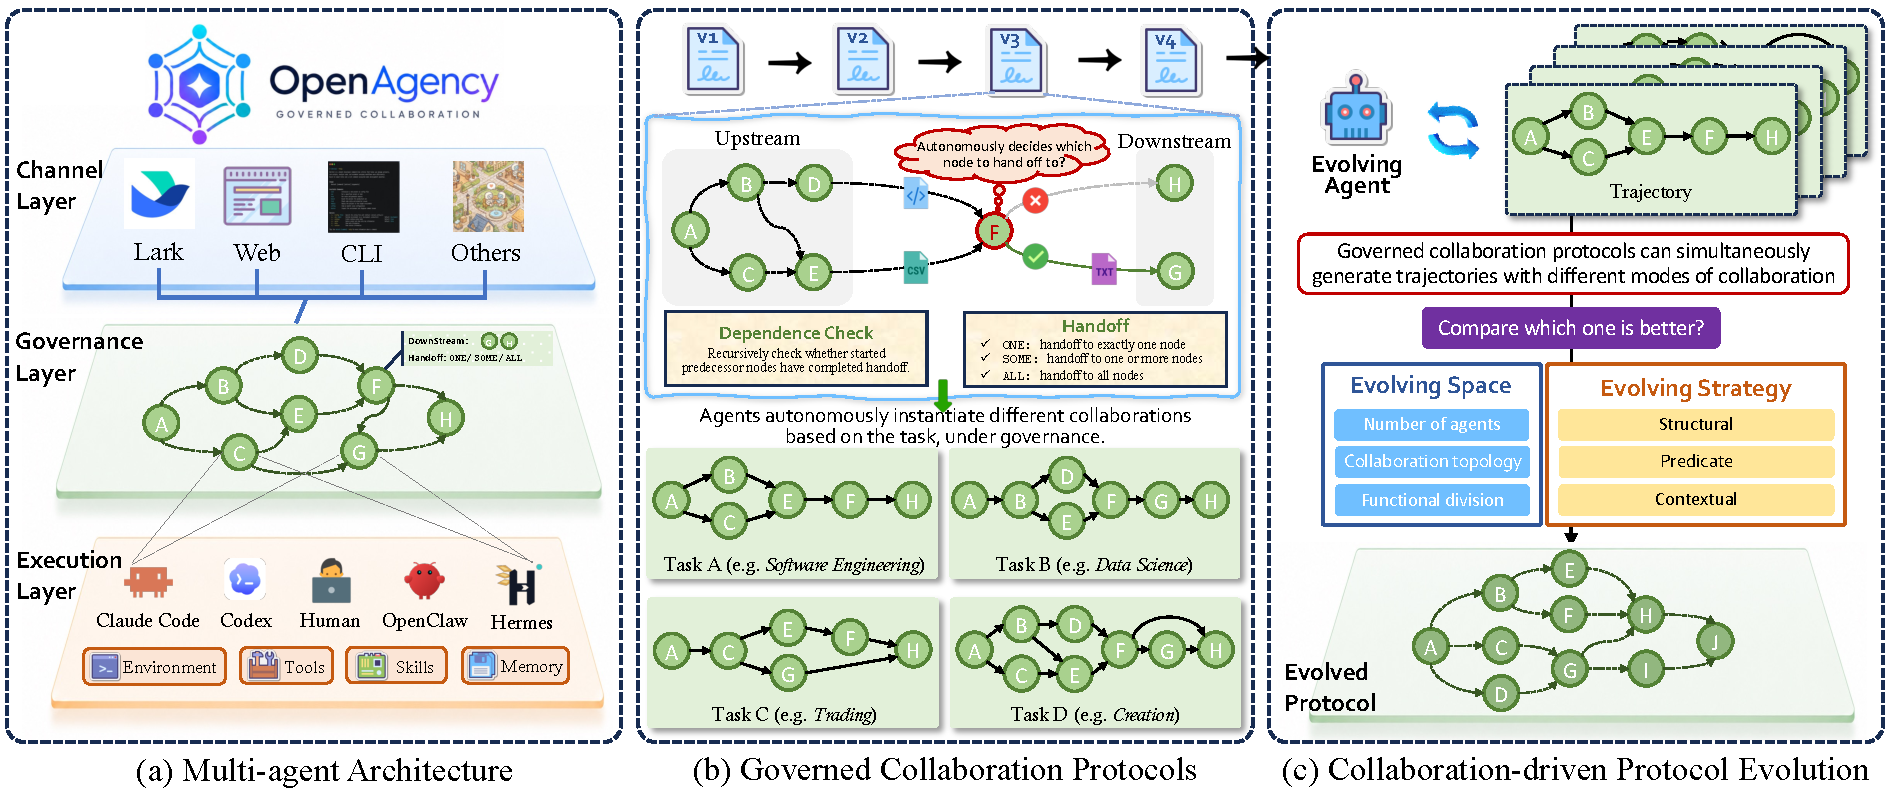
\includegraphics[width=0.99\linewidth]{figures/overview.pdf}
\caption{Overview of OpenAgency. (a) Three layers keep the collaboration protocol independent of the backend that realizes each role. (b) Under one governed protocol the agents choose their own handoffs, so different tasks instantiate different collaborations. (c) The evolving agent reads the collected trajectories and returns the next protocol, moving inside the evolving space under one of three edit strategies.}
\label{fig:intro}
\end{figure}

\section{OpenAgency}
\label{sec:method}

OpenAgency treats collaboration as a first-class object separated from the executors that realize each role. It combines a layered architecture (Section~\ref{sec:architecture}), a governed protocol that makes coordination inspectable (Section~\ref{sec:protocol}), and bounded protocol evolution driven by execution traces (Section~\ref{sec:self_evolving}), as Figure~\ref{fig:intro} illustrates.

\subsection{Multi-agent Architecture}
\label{sec:architecture}

To apply one collaboration protocol across applications with heterogeneous executors, OpenAgency separates multi-agent collaboration into three layers that keep the protocol independent of backend-specific prompts and actions.

\textbf{Channel Layer.}\quad The channel layer exposes the collaboration to its users through an enterprise chat workspace, a web console, or a command line, and keeps instructions, agent messages, human feedback, and coordination events on one shared timeline.

\textbf{Governance Layer.}\quad The governance layer hosts the collaboration protocol and validates each proposed handoff against the current protocol state. It records both accepted and rejected events in a trace that supplies the evidence for later protocol evolution.

\textbf{Execution Layer.}\quad The execution layer binds each role to a concrete executor. An executor can be an LLM agent, a coding harness, a domain-specific tool, or a human reviewer, and it sits below the governance layer, so the protocol constrains how roles hand off whichever backend realizes a role.

We formalize a running OpenAgency instance at step $t$ as $\mathcal{I}^{(t)} = (\mathcal{X}^{(t)}, \mathcal{P}, \mathcal{E}, s^{(t)})$, where $\mathcal{X}^{(t)}$ is the shared context, $\mathcal{P}$ is the governed protocol, $\mathcal{E}$ is the set of available executors, and $s^{(t)}$ is the current protocol state. The map $\rho: \mathcal{R}\rightarrow\mathcal{E}$ binds each role in the role set $\mathcal{R}$ to an executor and stays separate from the protocol logic. The governance layer renders the shared state into a role-specific execution context $u^{(t)} = f_{\mathrm{ctx}}(\mathcal{X}^{(t)}, s^{(t)}, n, r, \mathcal{P})$ for the active node $n$ with assigned role $r$, since an LLM executor may require tool instructions while a human executor may require a concise protocol description. Adapters return messages, handoffs, finishes, and failures in a common event format, so the executor bound to a role can change without changing the handoff rules, trace format, or completion predicates.

\subsection{Governed Collaboration Protocols}
\label{sec:protocol}

To govern collaboration without fixing a complete execution route, OpenAgency represents collaboration as a declarative tuple that exposes enough structure to validate each handoff while preserving the agent's choice among admissible targets.

\textbf{Protocol Definition.}\quad OpenAgency represents a governed collaboration protocol as
\begin{gather}
    \mathcal{P} = (\mathcal{R},\, \mathcal{N},\, \alpha,\, \mathcal{H},\, \mu,\, \Omega,\, \mathcal{C}),
\end{gather}
where $\mathcal{R}$ is the set of roles, $\mathcal{N}$ the set of collaboration nodes, $\alpha\colon \mathcal{N}\to\mathcal{R}$ assigns each node to a role, $\mathcal{H}\subseteq\mathcal{N}\times\mathcal{N}$ defines admissible handoff edges, $\mu(n)\in\{\texttt{ONE},\texttt{SOME},\texttt{ALL}\}$ is the handoff mode, $\Omega_n$ is the completion predicate, and $\mathcal{C}$ contains the shared \texttt{rule} and \texttt{culture} that every role sees.

\textbf{Admissible Handoff Set.}\quad For a node $n$ under state $s$, the admissible handoff set is $\Gamma(n,s) = \{\, n' \in \mathcal{N} \mid (n,n') \in \mathcal{H} \text{ and the transition is valid under } s \,\}$. The handoff mode $\mu(n)$ then determines how the active agent selects targets from $\Gamma(n,s)$. Under \texttt{ONE} the agent picks exactly one admissible target, under \texttt{SOME} a nonempty subset, and under \texttt{ALL} every admissible target. A node with no admissible target completes without a handoff, and the local choice within $\Gamma(n,s)$ is left to the agent.

\textbf{Handoff Validation and Completion.}\quad When the agent proposes a handoff $(n,B,m)$ with target set $B$ and message $m$, the protocol validates $B$ under $\mu(n)$. An admissible handoff commits $B$ as pending targets and updates the state, and an inadmissible one leaves the state unchanged and returns structured feedback so the agent may propose another target. Committing a target set does not activate it. A finish event $(n,y)$ reports the output $y$ that the source node produced, and the governance layer activates the committed targets only when the completion predicate $\Omega_n(y)$ holds on that output, so downstream execution waits for the completion predicate even after an admissible target set is committed. Activation runs one further dependence check, which walks back from each committed target and confirms that every started predecessor of that target has already handed off, so a node begins only once the collaborators it depends on have delivered.

Algorithm~\ref{alg:protocol} states the resulting runtime interpreter. The state advances only on admissible handoffs and valid completions, while the trace keeps every event, including the ones the boundary refused, so later evolution reads both successful and unsuccessful coordination.

\begin{algorithm}[t]
\footnotesize
\caption{Collaboration under a Governed Protocol}
\label{alg:protocol}
\begin{algorithmic}[1]
\renewcommand{\algorithmicrequire}{\textbf{Input:}}
\Require Protocol $\mathcal{P}$, initial context $\mathcal{X}$, executor mapping $\rho\colon\mathcal{R}\to\mathcal{E}$
\renewcommand{\algorithmicrequire}{\textbf{Output:}}
\Require Collaboration trace $\tau$

\State $\tau \gets \emptyset$; activate start node $n_0$; obtain initial state $s$
\While{active nodes exist}
    \For{each active node $n$ with role $r = \alpha(n)$}
        \State $e \gets \rho(r)\bigl(f_{\mathrm{ctx}}(\mathcal{X}, s, n, r, \mathcal{P})\bigr)$ \Comment{executor proposes an event}
        \If{$e$ is a handoff $(n, B, m)$ and $B$ is admissible}
            \State commit $B$ as pending targets and update $s$
        \ElsIf{$e$ is a finish $(n, y)$ and $\Omega_n(y)$ holds}
            \State mark $n$ complete, then activate every committed target whose started predecessors have handed off
        \Else
            \State return structured feedback to $\rho(r)$ \Comment{refused at the governance boundary}
        \EndIf
        \State append $(e, s)$ to $\tau$ \Comment{accepted and refused events are both retained}
    \EndFor
\EndWhile
\State \Return $\tau$
\end{algorithmic}
\end{algorithm}

\subsection{Collaboration-driven Protocol Evolution}
\label{sec:self_evolving}

Given a protocol whose decisions are explicit and checkable, the remaining question is how to revise it from experience. Revising a protocol takes the shape of an optimization problem, since it needs a signal that says where the current protocol is wrong, a space of admissible moves, and a rule that decides which move to keep. The final answer alone cannot indicate which of a run's many coordination events should change, and regenerating the whole workflow each round would destroy the governance boundary that makes a change inspectable. A single evolving agent therefore drives the loop. It reads a search direction off the collaboration trace, moves inside a bounded space of protocol edits, and keeps a move only when that move survives an admissibility and quality check.

\textbf{Trace Diagnosis as Search Signal.}\quad Each execution produces an ordered trace $\tau=(e_1,s_1),\ldots,(e_T,s_T)$ over the $T$ coordination events of that run and the states they produce, where an event $e_t$ is one of accepted handoff, rejected handoff, finish, message, or failure. Unlike prior systems that keep only the successful trajectory or the final score, the trace retains rejected handoffs and failed completions, which record the transitions the collaboration attempted and could not take. The evolving agent runs an analyzer $f_{\mathrm{diag}}$ over $\tau^{(1{:}v)}$, the traces collected in evolution rounds $1$ through $v$, and returns the coordination sites that account for the observed failures, namely the handoff edges the agents repeatedly attempted and the admissible set refused, together with the completion predicates that fired without a usable output. This signal plays the role a gradient plays in parameter optimization, since it attributes a run-level outcome to individual coordination decisions and points at the part of the protocol a revision should touch.

\textbf{Factorized Evolving Space.}\quad The search space factorizes into three levels. \emph{Number of agents} covers the node count $|\mathcal{N}|$. \emph{Collaboration topology} covers the handoff edge set $\mathcal{H}$ and the handoff modes $\mu$. \emph{Functional division} covers the role assignment $\alpha$, the completion predicates $\Omega$, and the shared \texttt{rule} and \texttt{culture} in $\mathcal{C}$, which together fix what each node owes the collaborators downstream of it. A point in this space is not one execution route, because each agent still chooses inside $\Gamma(n,s)$, so a single protocol unfolds into many realized collaboration patterns at inference time, as the four task instantiations of Figure~\ref{fig:intro} show. The optimizer therefore searches far fewer points than the collaborations they realize. The factorization also makes comparison readable, since a candidate produced by a single-level edit shares the remaining levels with the deployed protocol, so an overloaded role can be told apart from a missing edge.

\textbf{Bounded Protocol Optimizer.}\quad A move in this space is a composite edit of at most $k$ atomic changes drawn from three edit strategies. A \emph{structural} edit adds or removes a node or a handoff edge, a \emph{predicate} edit rewrites a completion or transition condition, and a \emph{contextual} edit rewrites the \texttt{rule} and \texttt{culture} a role reads. At round $v$ the optimizer $f_{\mathrm{evolve}}$ reads the deployed protocol $\mathcal{P}^{(v)}$ together with the analyzed trace signal and returns the edit set $\Delta^{(v)}$ to apply,
\begin{gather}
    \Delta^{(v)} = f_{\mathrm{evolve}}\bigl(\mathcal{P}^{(v)},\, f_{\mathrm{diag}}(\tau^{(1{:}v)})\bigr), \qquad \bigl|\Delta^{(v)}\bigr| \le k,
\end{gather}
where $\hat{\mathcal{P}}^{(v+1)}$ denotes the candidate obtained by applying $\Delta^{(v)}$ to $\mathcal{P}^{(v)}$, and the hat marks a candidate not yet checked.
We set $k=4$, which bounds the step the way a learning rate bounds a parameter update and keeps each candidate a small inspectable change. The strategy is a bounded greedy ascent, proposing one candidate per round and retaining the deployed protocol whenever the candidate fails the check below, so the deployed sequence never moves downhill in collaboration quality.

\textbf{Admissibility and Quality Check.}\quad A step is checked twice before it is deployed. The first check is a structural validity test $\Pi_{\mathcal{V}}$ on the candidate topology, which returns $1$ when the candidate is a well-formed protocol and $0$ when it carries malformed handoff edges, unresolved role references, duplicate node identifiers, or completion states no path can reach. The second check executes a candidate that passes the first one and hands the resulting traces to the evolving agent. The agent returns a collaboration quality score $q_{\mathrm{col}}$ from the realized coordination, reading whether each role delivered what its successors required and whether the completion conditions closed on a usable output. The deployment rule is
\begin{gather}
    \mathcal{P}^{(v+1)} =
    \begin{cases}
        \hat{\mathcal{P}}^{(v+1)}, & \Pi_{\mathcal{V}}\bigl(\hat{\mathcal{P}}^{(v+1)}\bigr) = 1 \;\text{ and }\; q_{\mathrm{col}}\bigl(\hat{\mathcal{P}}^{(v+1)}\bigr) \ge q_{\mathrm{col}}\bigl(\mathcal{P}^{(v)}\bigr),\\[2pt]
        \mathcal{P}^{(v)}, & \text{otherwise},
    \end{cases}
\end{gather}
the candidate is deployed only when it is well formed and does not degrade the observed coordination.

\section{Experiments}
\label{sec:experiments}

% We evaluate the governed protocol of Section~\ref{sec:method} on fourteen benchmarks (Section~\ref{sec:benchmarks}) under one executor and tool budget (Section~\ref{sec:setup}), and report the main comparison in Section~\ref{sec:main_results}. Section~\ref{sec:analysis} then locates the gain through the evolution rounds (Section~\ref{sec:evolution_effect}), their component measurements (Section~\ref{sec:subdim}), the agent count (Section~\ref{sec:ablation_multi}), the evolving space (Section~\ref{sec:ablation_space}), the free-form and SOP baselines (Section~\ref{sec:free_form}), the patterns one protocol reaches across tasks (Section~\ref{sec:admissible}), and a fixed graph (Section~\ref{sec:fixed_topology}).

\subsection{Benchmarks}
\label{sec:benchmarks}

We evaluate OpenAgency on fourteen benchmarks organized into three categories. \emph{General question answering} contains HumanEval~\citep{chen2021humaneval}, MBPP~\citep{austin2021mbpp}, GSM8K~\citep{cobbe2021gsm8k}, MATH~\citep{hendrycks2021math}, and HotpotQA~\citep{yang2018hotpotqa}, and tests protocol adaptation when each instance admits a short answer. \emph{Long-horizon tasks} contains SWE-bench Verified~\citep{jimenez2024swebench}, DeepPlanning~\citep{zhang2026deepplanning}, and the text-only subset of Humanity's Last Exam (HLE), and tests governed handoffs on dependent decisions. \emph{Production-oriented tasks} contains DevEval~\citep{li2024deveval}, DDR-Bench~\citep{liu2026ddrbench}, TheAgentCompany~\citep{xu2024theagentcompany}, MARBLE~\citep{zhu2025marble}, AutomationBench~\citep{shepard2026automationbench}, and OfficeQA Pro~\citep{opsahlong2026officeqa}, and tests one protocol across heterogeneous tools and task formats. Appendix~\ref{app:benchmarks} describes each benchmark.

\subsection{Experimental Setup}
\label{sec:setup}

To separate governed collaboration from the executor's own capability, we use GPT-5.5 across all benchmarks, and each role receives the tools its benchmark requires. For each benchmark, we compare three in-house conditions, a single-agent ablation with no handoff, the unstructured initialization $v_0$, and the evolved protocol after four rounds ($v_4$). All three are reported against a prior system (Prior Sys.), the best of the officially reported results and our GPT-5.5 implementation for each benchmark at submission time. Each benchmark evolves its own protocol, and the evolving agent reads only execution traces, so no task label or reference answer reaches it, following the label-free self-refinement setting of \citet{shinn2023reflexion} and \citet{madaan2023selfrefine}. Model, temperature, and tool budget stay fixed across rounds, and only the protocol changes. Table~\ref{tab:main} reports the final round and Appendix~\ref{app:detail} lists all four.

\subsection{Main Results}
\label{sec:main_results}

% \begin{wrapfigure}{r}{0.44\textwidth}
% \vspace{-6mm}
% \centering
% 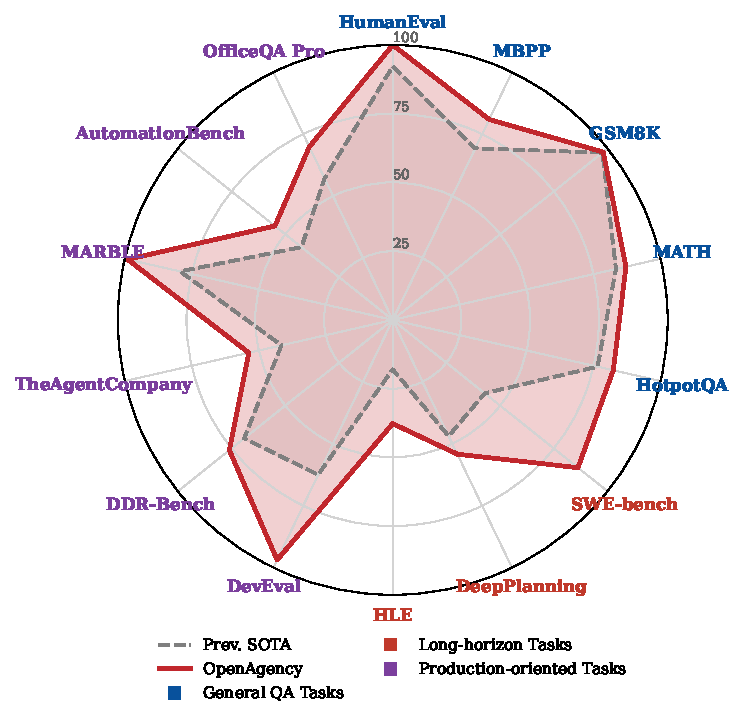
\includegraphics[width=0.7\linewidth]{figures/main_radar.pdf}
% \vspace{-4mm}
% \caption{OpenAgency against each benchmark's prior system across three categories. The same protocol runs on all fourteen benchmarks.}
% \label{fig:main_radar}
% \vspace{-4mm}
% \end{wrapfigure}
\begin{table}[t]
\caption{Results of OpenAgency on each benchmark. Prior Sys. is the best of the officially reported results and our GPT-5.5 implementation for each benchmark. Multi-agent~(init) is the unstructured initialization and OpenAgency is the evolved protocol, both sharing the GPT-5.5 backbone. Each row uses the benchmark's native metric, where EM is exact match, FM is file match, and AT is the acceptance-test pass rate.}
\label{tab:main}
\begin{center}
\small
\setlength{\tabcolsep}{5pt}
\begin{tabular}{llcccc}
\toprule
\textbf{Benchmark} & \textbf{Metric} & \textbf{Prior Sys.} & \textbf{Single-agent} & \textbf{Multi-agent (init)} & \textbf{OpenAgency} \\
\midrule
\multicolumn{6}{c}{\emph{General Question Answering Tasks}} \\
HumanEval & pass@1 & 92.2 & 87.5 & 96.9 & \textbf{100.0} \\
MBPP & pass@1 & 69.3 & 73.5 & 73.5 & \textbf{80.9} \\
GSM8K & EM & 97.6 & 97.2 & 97.4 & \textbf{98.0} \\
MATH & EM & 83.3 & 82.3 & 86.0 & \textbf{87.0} \\
HotpotQA & F1 & 76.4 & 75.9 & 64.0 & \textbf{82.3} \\
\midrule
\multicolumn{6}{c}{\emph{Long-horizon Tasks}} \\
SWE-bench Verified & FM & 42.8 & 75.6 & 67.0 & \textbf{86.2} \\
DeepPlanning & Case Acc & 46.9 & 45.0 & 33.8 & \textbf{54.2} \\
HLE (text-only) & Accuracy & 18.0 & 18.4 & 5.6 & \textbf{37.7} \\
\midrule
\multicolumn{6}{c}{\emph{Production-oriented Tasks}} \\
DevEval & AT & 62.5 & 62.5 & 82.1 & \textbf{96.9} \\
DDR-Bench & Overall & 69.1 & 42.8 & 44.0 & \textbf{76.0} \\
TheAgentCompany & Score & 41.5 & 46.3 & 41.5 & \textbf{53.7} \\
MARBLE & Overall & 79.3 & 78.4 & 50.0 & \textbf{98.9} \\
AutomationBench & Acc & 42.5 & 23.7 & 23.6 & \textbf{54.8} \\
OfficeQA Pro & Acc@1\% & 57.1 & 35.3 & 21.1 & \textbf{69.9} \\
\bottomrule
\end{tabular}
\end{center}
\vspace{-2mm}
\end{table}

\textbf{Capability on General Question Answering.}\quad The five single-turn benchmarks probe \emph{short-chain reasoning capabilities}, since each instance has a localized, automatically verifiable output. As shown in Table~\ref{tab:main}, OpenAgency obtains the best primary metric on all five, reaching $100.0$ pass@1 on HumanEval and lifting MBPP from $73.5$ to $80.9$ over the initialization. Agent count alone does not produce this gain, since the initialization trails the single-agent ablation on HotpotQA at $64.0$ against $75.9$ F1 while the governed protocol reaches $82.3$. Evolution prunes handoffs whose upstream output the trace flags as ineffective, and each benchmark settles on a solve-critique-revise loop matched to its dominant failure mode. Overall, OpenAgency's strong results here highlight its capability to reshape a protocol even where a short answer suffices.

\textbf{Capability on Long-horizon Tasks.}\quad SWE-bench Verified, DeepPlanning, and HLE stress \emph{long-horizon reasoning capabilities}, since a bad handoff at any stage can invalidate the entire run. Table~\ref{tab:main} reports a lead on all three, reaching $86.2$ file match on SWE-bench Verified against a prior system of $42.8$ and $37.7$ accuracy on HLE. More importantly, the protocol each benchmark converges to shows why. On SWE-bench Verified the evolving agent installs a retry edge when a patch fails and splits an overloaded Verifier into structural and semantic components, DeepPlanning hands its Verifier the constraints one at a time, and HLE makes verification conditional on answer confidence. All three shapes come from the same initialization, so the handoff and completion rules adapt when local errors are unrecoverable. Overall, OpenAgency's strong results here highlight its capability to keep dependent decisions recoverable.

\textbf{Capability on Production-oriented Tasks.}\quad The six production-oriented benchmarks test \emph{cross-domain deployment capabilities}, since each exposes a different set of tools. As shown in Table~\ref{tab:main}, OpenAgency leads on all six, improving over the prior system by $34.4$ points on DevEval, $19.6$ points on MARBLE, and $12.8$ points on OfficeQA Pro. The template differs per benchmark, and in particular two cases expose what governance contributes. On DDR-Bench, an Auditor role introduced during evolution forces every quantitative finding in the trace into the final report, fixing a silent omission free-form baselines leave undetected. The admissible-set constraint on MARBLE keeps each handoff terminating where any-to-any messaging would not, so governance supplies a constraint the task format alone does not. Overall, OpenAgency's strong results here highlight its capability to carry one governed protocol across heterogeneous tools.

\section{Analysis}
\label{sec:analysis}

\subsection{Effectiveness of Protocol Evolution}
\label{sec:evolution_effect}

To verify that bounded edits keep improving collaboration after the first revision, we track the primary metric from the initialization $v_0$ to the evolved rounds $v_1$ through $v_4$ on all fourteen benchmarks. Figure~\ref{fig:evolution} and Table~\ref{tab:evolution_all} record an improvement over the initialization on every benchmark, reaching $48.9$ points on MARBLE and $48.8$ points on OfficeQA Pro. The deployed sequence is non-decreasing in collaboration quality, since the check keeps the deployed protocol whenever a candidate scores lower, and on these fourteen benchmarks the ordering also holds for the primary task metric.

\begin{figure}[t]
\centering
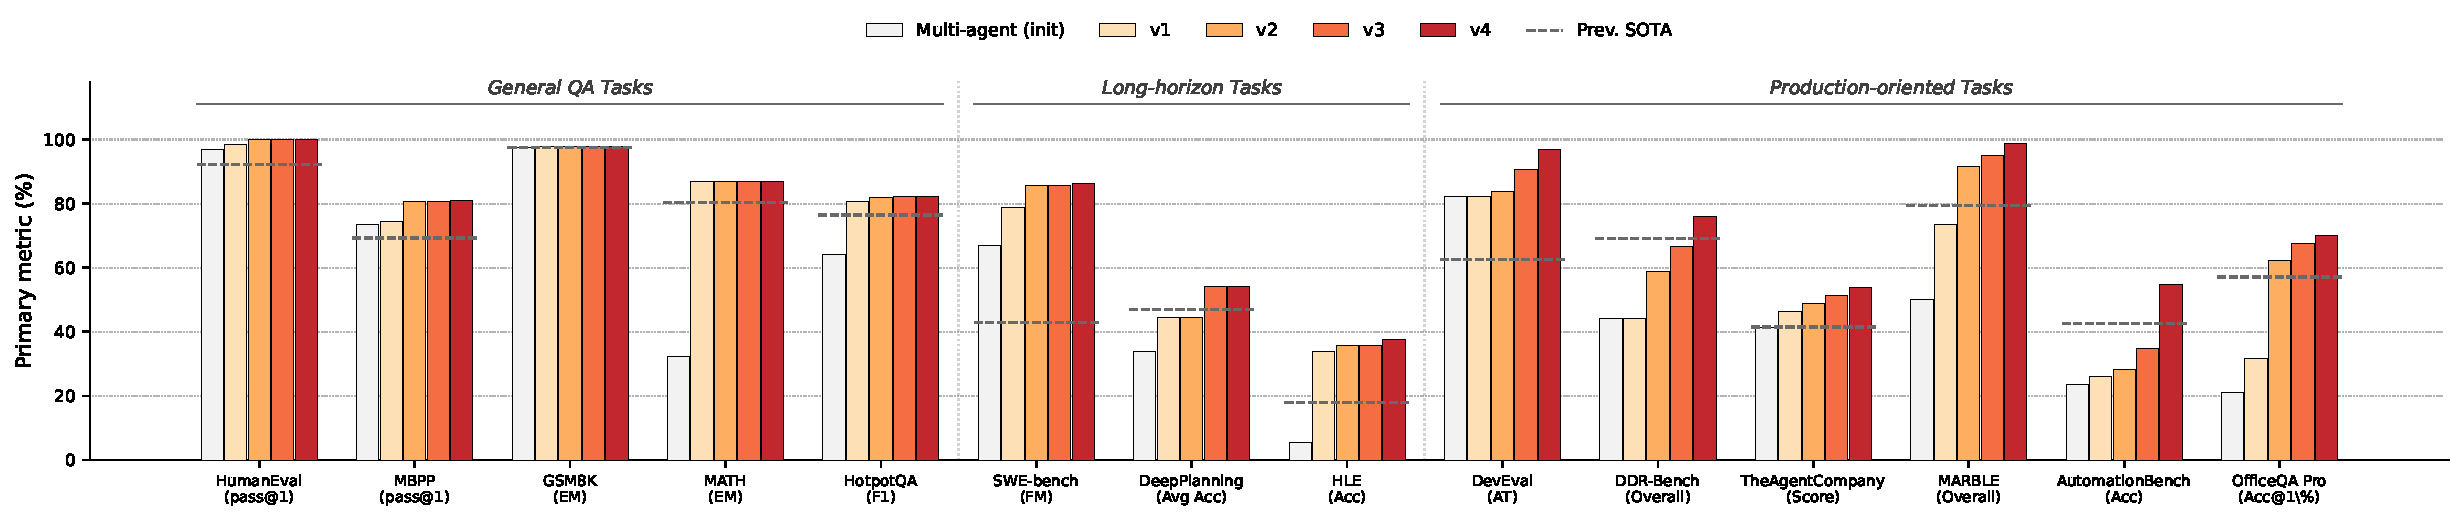
\includegraphics[width=0.98\linewidth]{figures/evolution_bars.pdf}
\vspace{-2mm}
\caption{Round-wise trajectory of the primary metric from the initialization $v_0$ through the evolved rounds $v_1$--$v_4$. Grey dashed lines mark each benchmark's prior system.}
\label{fig:evolution}
\end{figure}

\subsection{Detailed Improvement across Evolution}
\label{sec:subdim}


\begin{wraptable}{r}{0.47\textwidth}
\vspace{-6mm}
\caption{Improvements across evolution.}
\vspace{1mm}
\label{tab:subdim}
\centering
\small
\setlength{\tabcolsep}{2pt}
\begin{tabular}{lccccc}
\toprule
\textbf{Component} & \textbf{Init} & $v_1$ & $v_2$ & $v_3$ & $v_4$ \\
\midrule
\multicolumn{6}{c}{\emph{SWE-bench Verified}} \\
Patch applied & 79.2 & 93.4 & 100.0 & 100.0 & \textbf{100.0} \\
File match & 67.0 & 78.8 & 85.6 & 85.8 & \textbf{86.2} \\
FM given a patch & 84.6 & 84.4 & 85.6 & 85.8 & \textbf{86.2} \\
\midrule
\multicolumn{6}{c}{\emph{DevEval}} \\
Unit test & 98.1 & 98.1 & 97.3 & 99.1 & \textbf{99.1} \\
Acceptance test & 82.1 & 82.1 & 83.9 & 90.6 & \textbf{96.9} \\
\bottomrule
\vspace{-7mm}
\end{tabular}
\end{wraptable}
To locate the gain inside a benchmark, we decompose the SWE-bench Verified and DevEval results of every round into their component measurements. As shown in Table~\ref{tab:subdim}, the two improve at different points. On SWE-bench Verified the file-match rate given a patch moves only from $84.6$ to $86.2$, while the fraction of instances producing a patch at all rises from $79.2$ to $100.0$, so the gain is consistent with closing the no-output failure mode that the retry edges of Section~\ref{sec:self_evolving} target. On DevEval the unit-test rate stays near saturation while acceptance rises from $82.1$ to $96.9$, so the admitted edits track the repository-level correctness that unit tests leave unchecked.

\begin{figure}[t]
\centering
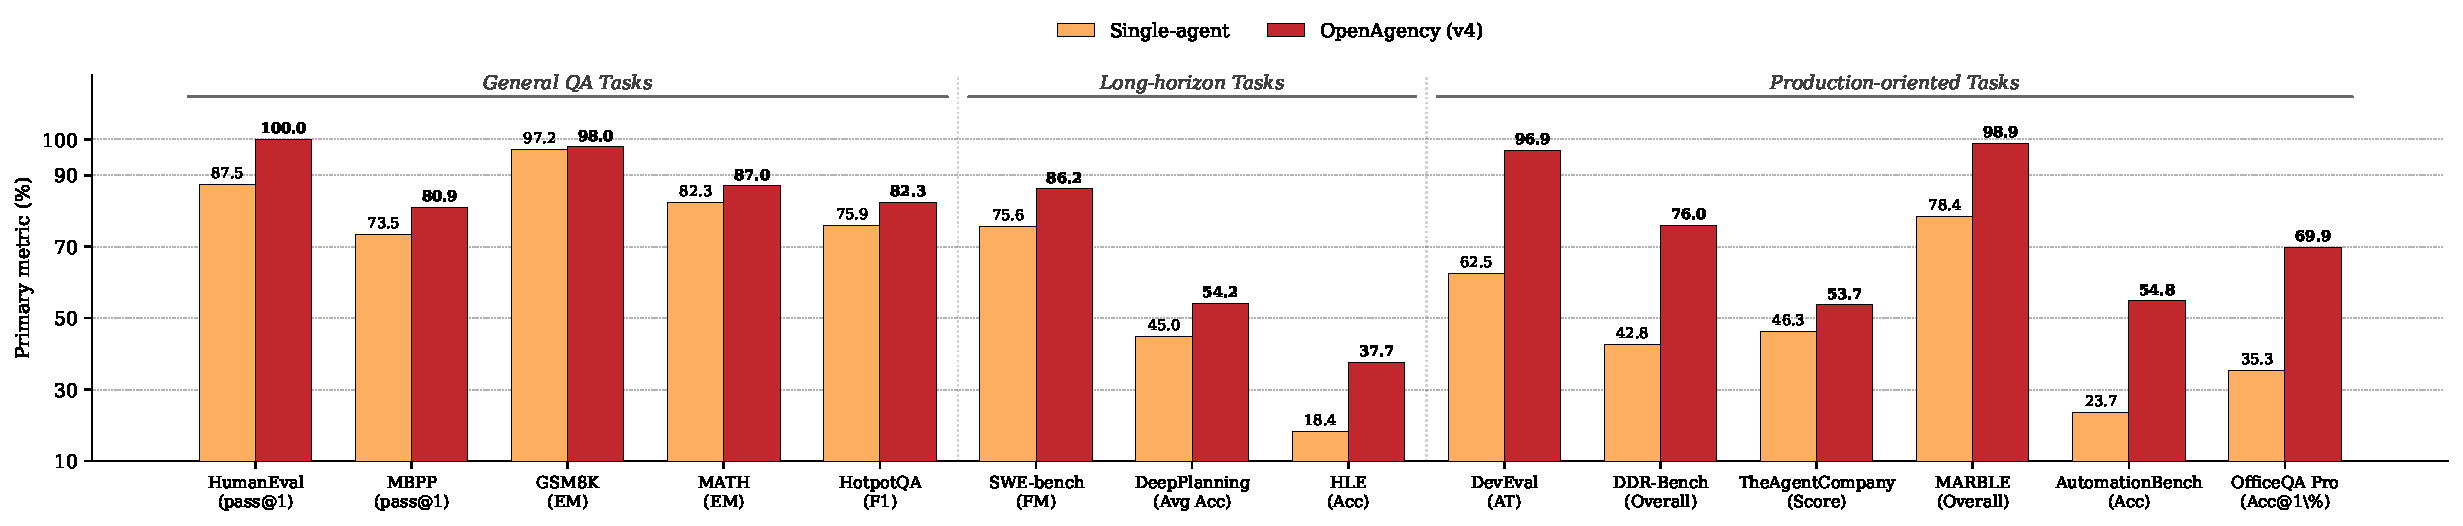
\includegraphics[width=0.99\linewidth]{figures/single_vs_multi.pdf}
\caption{OpenAgency versus its single-agent ablation under one model and tool budget.}
\label{fig:svm}
\end{figure}



\subsection{Ablation of Evolving Space}
\label{sec:ablation_space}

\begin{wrapfigure}{r}{0.4\textwidth}
\vspace{-10mm}
\centering
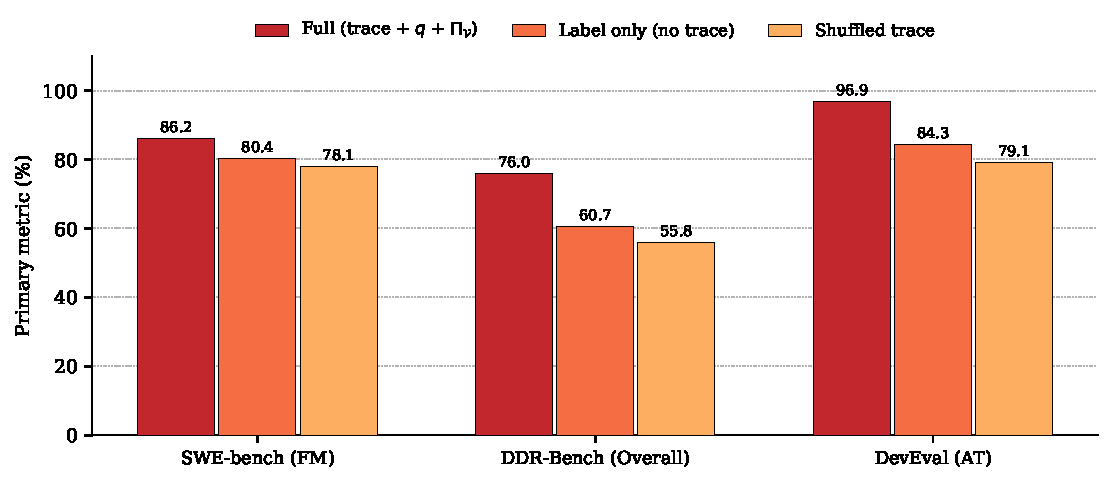
\includegraphics[width=\linewidth]{figures/evolution_ablation.pdf}
\vspace{-4mm}
\caption{Effect of three evolving spaces. The fixed-count setting holds the agent number, and the division-only setting freezes the whole graph.}
\vspace{-3mm}
\label{fig:evo_space}
\end{wrapfigure}
To identify which levels of the evolving space carry the gain, we restrict that space in two nested steps and rerun the same evolution loop on three benchmarks. The full setting edits all three levels of Section~\ref{sec:self_evolving}, the fixed-count setting holds the agent count $|\mathcal{N}|$, and the division-only setting freezes the whole graph. Figure~\ref{fig:evo_space} reports the best protocol each setting reaches, and the three benchmarks order the three settings identically. Freezing the agent count alone costs $5.8$ points on SWE-bench Verified, $12.6$ on DevEval, and $15.3$ on DDR-Bench, so the freedom to change the agent count is the level that contributes most, and freezing the remaining handoff structure costs a further $2.3$ to $5.2$ points. In essence, a hand-designed system commits both structural levels before reading any trace.

\subsection{Comparison against Free-form and SOP Baselines}
\label{sec:free_form}

\begin{wraptable}{r}{0.47\textwidth}
\vspace{-4mm}
\caption{Results of OpenAgency against the free-form and SOP baselines.}
\vspace{2mm}
\label{tab:free_form}
\centering
\small
\setlength{\tabcolsep}{2.5pt}
\begin{tabular}{lcccc}
\toprule
\textbf{System} & \textbf{SWE-} & \textbf{Dev} & \textbf{DDR-} & \textbf{TheAgent} \\
 & \textbf{bench} & \textbf{Eval} & \textbf{Bench} & \textbf{Company} \\
\midrule
AutoGen & 51.4 & 68.9 & 39.2 & 38.7 \\
ChatDev & 57.6 & 78.3 & 44.1 & 41.9 \\
MetaGPT & 59.8 & 79.5 & 46.8 & 42.3 \\
\rowcolor{gray!12}
\textbf{OpenAgency} & \textbf{86.2} & \textbf{96.9} & \textbf{76.0} & \textbf{53.7} \\
\bottomrule
\end{tabular}
\end{wraptable}
To compare the three ways of expressing collaboration, we evaluate OpenAgency against the free-form baseline AutoGen \citep{wu2023autogenenablingnextgenllm} and the SOP baselines ChatDev \citep{qian2024chatdevcommunicativeagentssoftware} and MetaGPT \citep{hong2024metagptmetaprogrammingmultiagent}. As shown in Table~\ref{tab:free_form}, OpenAgency obtains the highest score, exceeding the strongest SOP baseline by $26.4$ points on SWE-bench Verified. Notably, the free-form baseline is the weakest everywhere, and the SOP baselines recover part of the gap because the collaboration order is enforced, yet their fixed procedure absorbs no trace-level failure signal.

\subsection{Advantage of Multi-agent Protocols}
\label{sec:ablation_multi}

To attribute the gain to governance and not to agent count, we compare OpenAgency with its single-agent ablation under one GPT-5.5 executor and identical tool access. As shown in Figure~\ref{fig:svm}, OpenAgency exceeds that ablation on every benchmark, with the widest gaps on OfficeQA Pro, DevEval, and DDR-Bench. A single node interleaves solving and checking inside one context, while the governed protocol routes a partial output to a downstream role that validates it independently. The initialization column of Table~\ref{tab:main} agrees, since a multi-agent initialization without a governed protocol falls short.

\subsection{Flexibility of Governed Protocols across Tasks}
\label{sec:admissible}

\begin{wraptable}{r}{0.44\textwidth}
\vspace{-\intextsep}
\caption{Governance activity on three deployed $v_4$ protocols with different handoff chains, as the share of proposed handoffs $\Gamma(n,s)$ rules out and the share of runs whose outcome that refusal changes.}
\vspace{2mm}
\label{tab:handoff}
\centering
\small
\setlength{\tabcolsep}{4pt}
\begin{tabular}{lccc}
\toprule
 & \textbf{Dev} & \textbf{DDR-} & \textbf{TheAgent} \\
 & \textbf{Eval} & \textbf{Bench} & \textbf{Company} \\
\midrule
Agents        & 2 & 2 & 3 \\
Refused (\%)   & 4.9 & 3.8 & 8.2 \\
Recovered (\%) & 3.7 & 2.9 & 5.3 \\
\bottomrule
\end{tabular}
\end{wraptable}
To show what one governed protocol deploys once the task changes, we read out the deployed $v_4$ protocol on three production-oriented benchmarks. As shown in Table~\ref{tab:handoff}, the three protocols differ in agent count, role vocabulary, and handoff order. DevEval converges on a coder checked by a reviewer, DDR-Bench on a researcher feeding a reporter, and TheAgentCompany on a planner, an executor, and a reviewer, so one loop settles on the division each task rewards. The admissible handoff set stays active on all three chains, ruling out $3.8\%$ to $8.2\%$ of proposed handoffs and changing the outcome of $2.9\%$ to $5.3\%$ of runs. A fixed procedure commits to one of these patterns before any trace is seen, and the refused events are the evidence the evolving agent consumes in Section~\ref{sec:self_evolving}.

\subsection{Superiority of Governed Protocols for Evolution}
\label{sec:fixed_topology}

% \begin{wrapfigure}{r}{0.45\textwidth}
% \vspace{-\intextsep}
% \centering
% 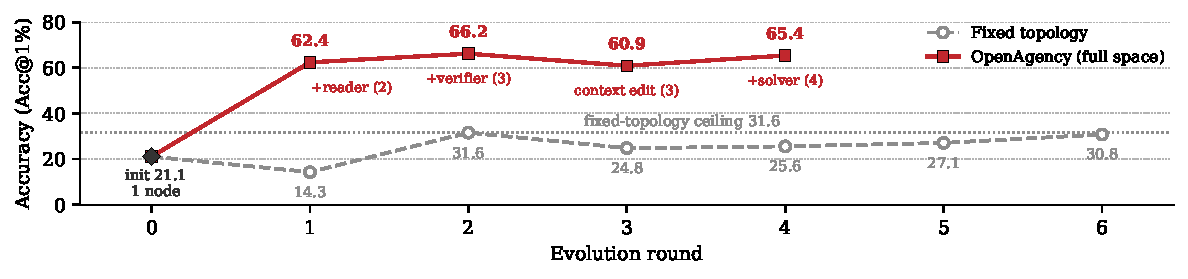
\includegraphics[width=\linewidth]{figures/fixed_topology.pdf}
% \caption{Evolution on OfficeQA Pro from one initialization, scored on the same $133$ tasks.}
% \label{fig:fixed}
% \end{wrapfigure}

\begin{figure}
    \centering
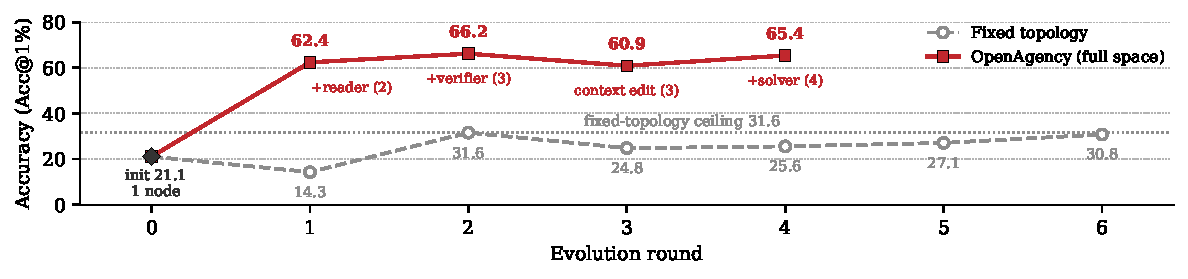
\includegraphics[width=\linewidth]{figures/fixed_topology.pdf}
    \vspace{-3mm}
    \caption{Evolution of OpenAgency and MetaGPT on OfficeQA Pro.}
\label{fig:fixed}
\end{figure}

To measure what a fixed collaboration graph costs, we plot the OfficeQA Pro evolution record under two settings from one initialization. The previous-protocol setting applies MetaGPT~\citep{hong2024metagptmetaprogrammingmultiagent} and rewrites only the functional division over a single-node graph. As shown in Figure~\ref{fig:fixed}, six such rewrites peak at $31.6$ in round $2$, and the four later ones fall back below it. The full setting, which may also change the agent count and the handoff structure, reaches $62.4$ once a reader node is added and $69.9$ after four rounds, matching Table~\ref{tab:evolution_all}. Both settings share the executor, the tool budget, and the $133$ scored tasks, so the gap comes from the level an edit may reach. A fixed graph keeps the search inside a level the trace already reports as saturated, and one structural edit clears that ceiling by more than thirty points.

\section{Conclusion}

We introduced OpenAgency, a self-evolving multi-agent system whose governed collaboration protocol makes the collaboration pattern an evolvable object, updated from ordered traces under a validity check. Experiments on fourteen benchmarks show that OpenAgency leads the compared systems on every primary metric, and that the gain keeps accumulating across the evolution rounds.

\subsection*{AI use statement}

In this work, we used generative AI tools only for final-stage language polishing and grammar refinement of the manuscript. We have not used generative AI tools for generating research ideas, designing methods, conducting experiments, implementing code, analyzing data, interpreting results, or producing scientific claims, and other generative AI-assisted tasks requiring disclosure are not applicable to this work. We have reviewed all AI-assisted revisions to ensure their correctness and consistency with the authors' intended content. We take responsibility for the final content of this work, including all text, claims, and artifacts produced with the aid of generative AI.

\subsection*{Reproducibility statement}

We have made efforts to ensure the reproducibility of this work by providing detailed descriptions of the proposed method, experimental settings, implementation details, and evaluation protocols in the main paper and supplementary materials. The supplementary materials include the source code required to reproduce our experiments, and we will publicly release the code after the review process to further facilitate verification and future research. The content of this paper can be completely reproduced.

\bibliography{iclr2027_conference}
\bibliographystyle{iclr2027_conference}

\appendix

\clearpage
\section{Benchmark Details}
\label{app:benchmarks}

\textbf{HumanEval}~\citep{chen2021humaneval} evaluates function-level Python code synthesis from natural-language docstrings.

\textbf{MBPP}~\citep{austin2021mbpp} evaluates short-form program synthesis from natural-language descriptions.

\textbf{GSM8K}~\citep{cobbe2021gsm8k} evaluates multi-step reasoning over grade-school math word problems.

\textbf{MATH}~\citep{hendrycks2021math} evaluates competition-level mathematical reasoning across five subject areas.

\textbf{HotpotQA}~\citep{yang2018hotpotqa} evaluates multi-hop question answering that links evidence from multiple documents.

\textbf{SWE-bench Verified}~\citep{jimenez2024swebench} evaluates repository-level software repair on human-validated GitHub issues, where the agent must produce a patch that resolves the reported bug against a hidden test suite.

\textbf{DeepPlanning}~\citep{zhang2026deepplanning} evaluates travel and shopping planning under user-specified constraints, and the primary metric is mean case-level accuracy across the two task families.

\textbf{Humanity's Last Exam (HLE)} evaluates expert-level question answering across mathematics, physics, biology, humanities, computer science, and engineering, and we use its 2{,}158-question text-only subset.

\textbf{DevEval}~\citep{li2024deveval} evaluates repository-level code generation under acceptance-test oracles that check whether the generated code works end-to-end with existing modules.

\textbf{DDR-Bench}~\citep{liu2026ddrbench} evaluates deep data research over 10-K SEC filings, and the overall metric averages message-wise correctness (per-question factuality) and trajectory-wise correctness (multi-turn consistency).

\textbf{TheAgentCompany}~\citep{xu2024theagentcompany} evaluates end-to-end task completion in a simulated enterprise environment, where each task requires a full containerized stack.

\textbf{MARBLE}~\citep{zhu2025marble} evaluates open-ended research and buyer-seller negotiation under rubric-based scores within the MultiAgentBench framework.

\textbf{AutomationBench}~\citep{shepard2026automationbench} evaluates cross-application business-workflow orchestration through REST APIs, and the primary metric is accuracy across its 600 tasks.

\textbf{OfficeQA Pro}~\citep{opsahlong2026officeqa} evaluates enterprise-grade grounded numerical reasoning over the U.S. Treasury Bulletin corpus, with correctness scored under a $1\%$ numerical tolerance.

\section{Case Study of Protocol Evolution}
\label{app:case_study}

Figure~\ref{fig:case_evo} shows how the protocol evolves across rounds on the nine long-horizon and production-oriented benchmarks, which jointly cover repository-level coding, planning, retrieval, workflow orchestration, and open-ended research. On every benchmark the number of nodes remains small ($\leq 4$ across rounds), so evolution acts as a rewiring process over a protocol that stays small across very different tasks.

The three edit levels are unevenly used. Structural edits dominate, appearing in $22$ of the $27$ revisions in Figure~\ref{fig:case_evo}, and the remaining five revise a predicate or the shared context without touching the graph. DevEval is the clearest case, where the second round moves unit-test injection into the shared rule and the third round bounds the review loop and records known error patterns, both without adding a role. Both rounds change how the protocol behaves while leaving the graph fixed, which a static topology has no place to record.

On the coding and planning benchmarks, evolution mainly redistributes verification responsibility. The SWE-bench Verified protocol first attaches a retry edge from the Verifier back to the Editor, then re-routes the Verifier back to the Locator, and finally splits the Verifier into structural and semantic components. DevEval gains a self-test node between the Coder and the Reviewer. DeepPlanning grows from a monolithic solver into a Researcher-Solver-Verifier chain with an explicit constraint checklist.

On the retrieval and research benchmarks, evolution adds evidence-preserving roles. The DDR-Bench protocol fixes the Researcher-to-Reporter handoff to forward the raw evidence set, splits a single reporting phase into two, and installs a quantitative Auditor. OfficeQA Pro converts a monolithic solver into a Reader-Solver-Verifier chain over an external document store. MARBLE replaces the initial Reviewer-Brainstormer-Writer handoff with a compact Generator-Critic-Reviser pipeline and adds a feasibility-driven retry edge from the Critic back to the Generator.

Evolution also shrinks the graph when coordination is unnecessary. AutomationBench collapses a two-node Executor-Verifier pipeline into a single-node solver with progressively tightened internal phases, while HLE grows a confidence-routed subgraph that skips verification on high-confidence answers and adds a retry edge on refused ones. Section~\ref{sec:subdim} locates the component measurement on which the accepted edits pay off.

\begin{figure}[!ht]
\centering
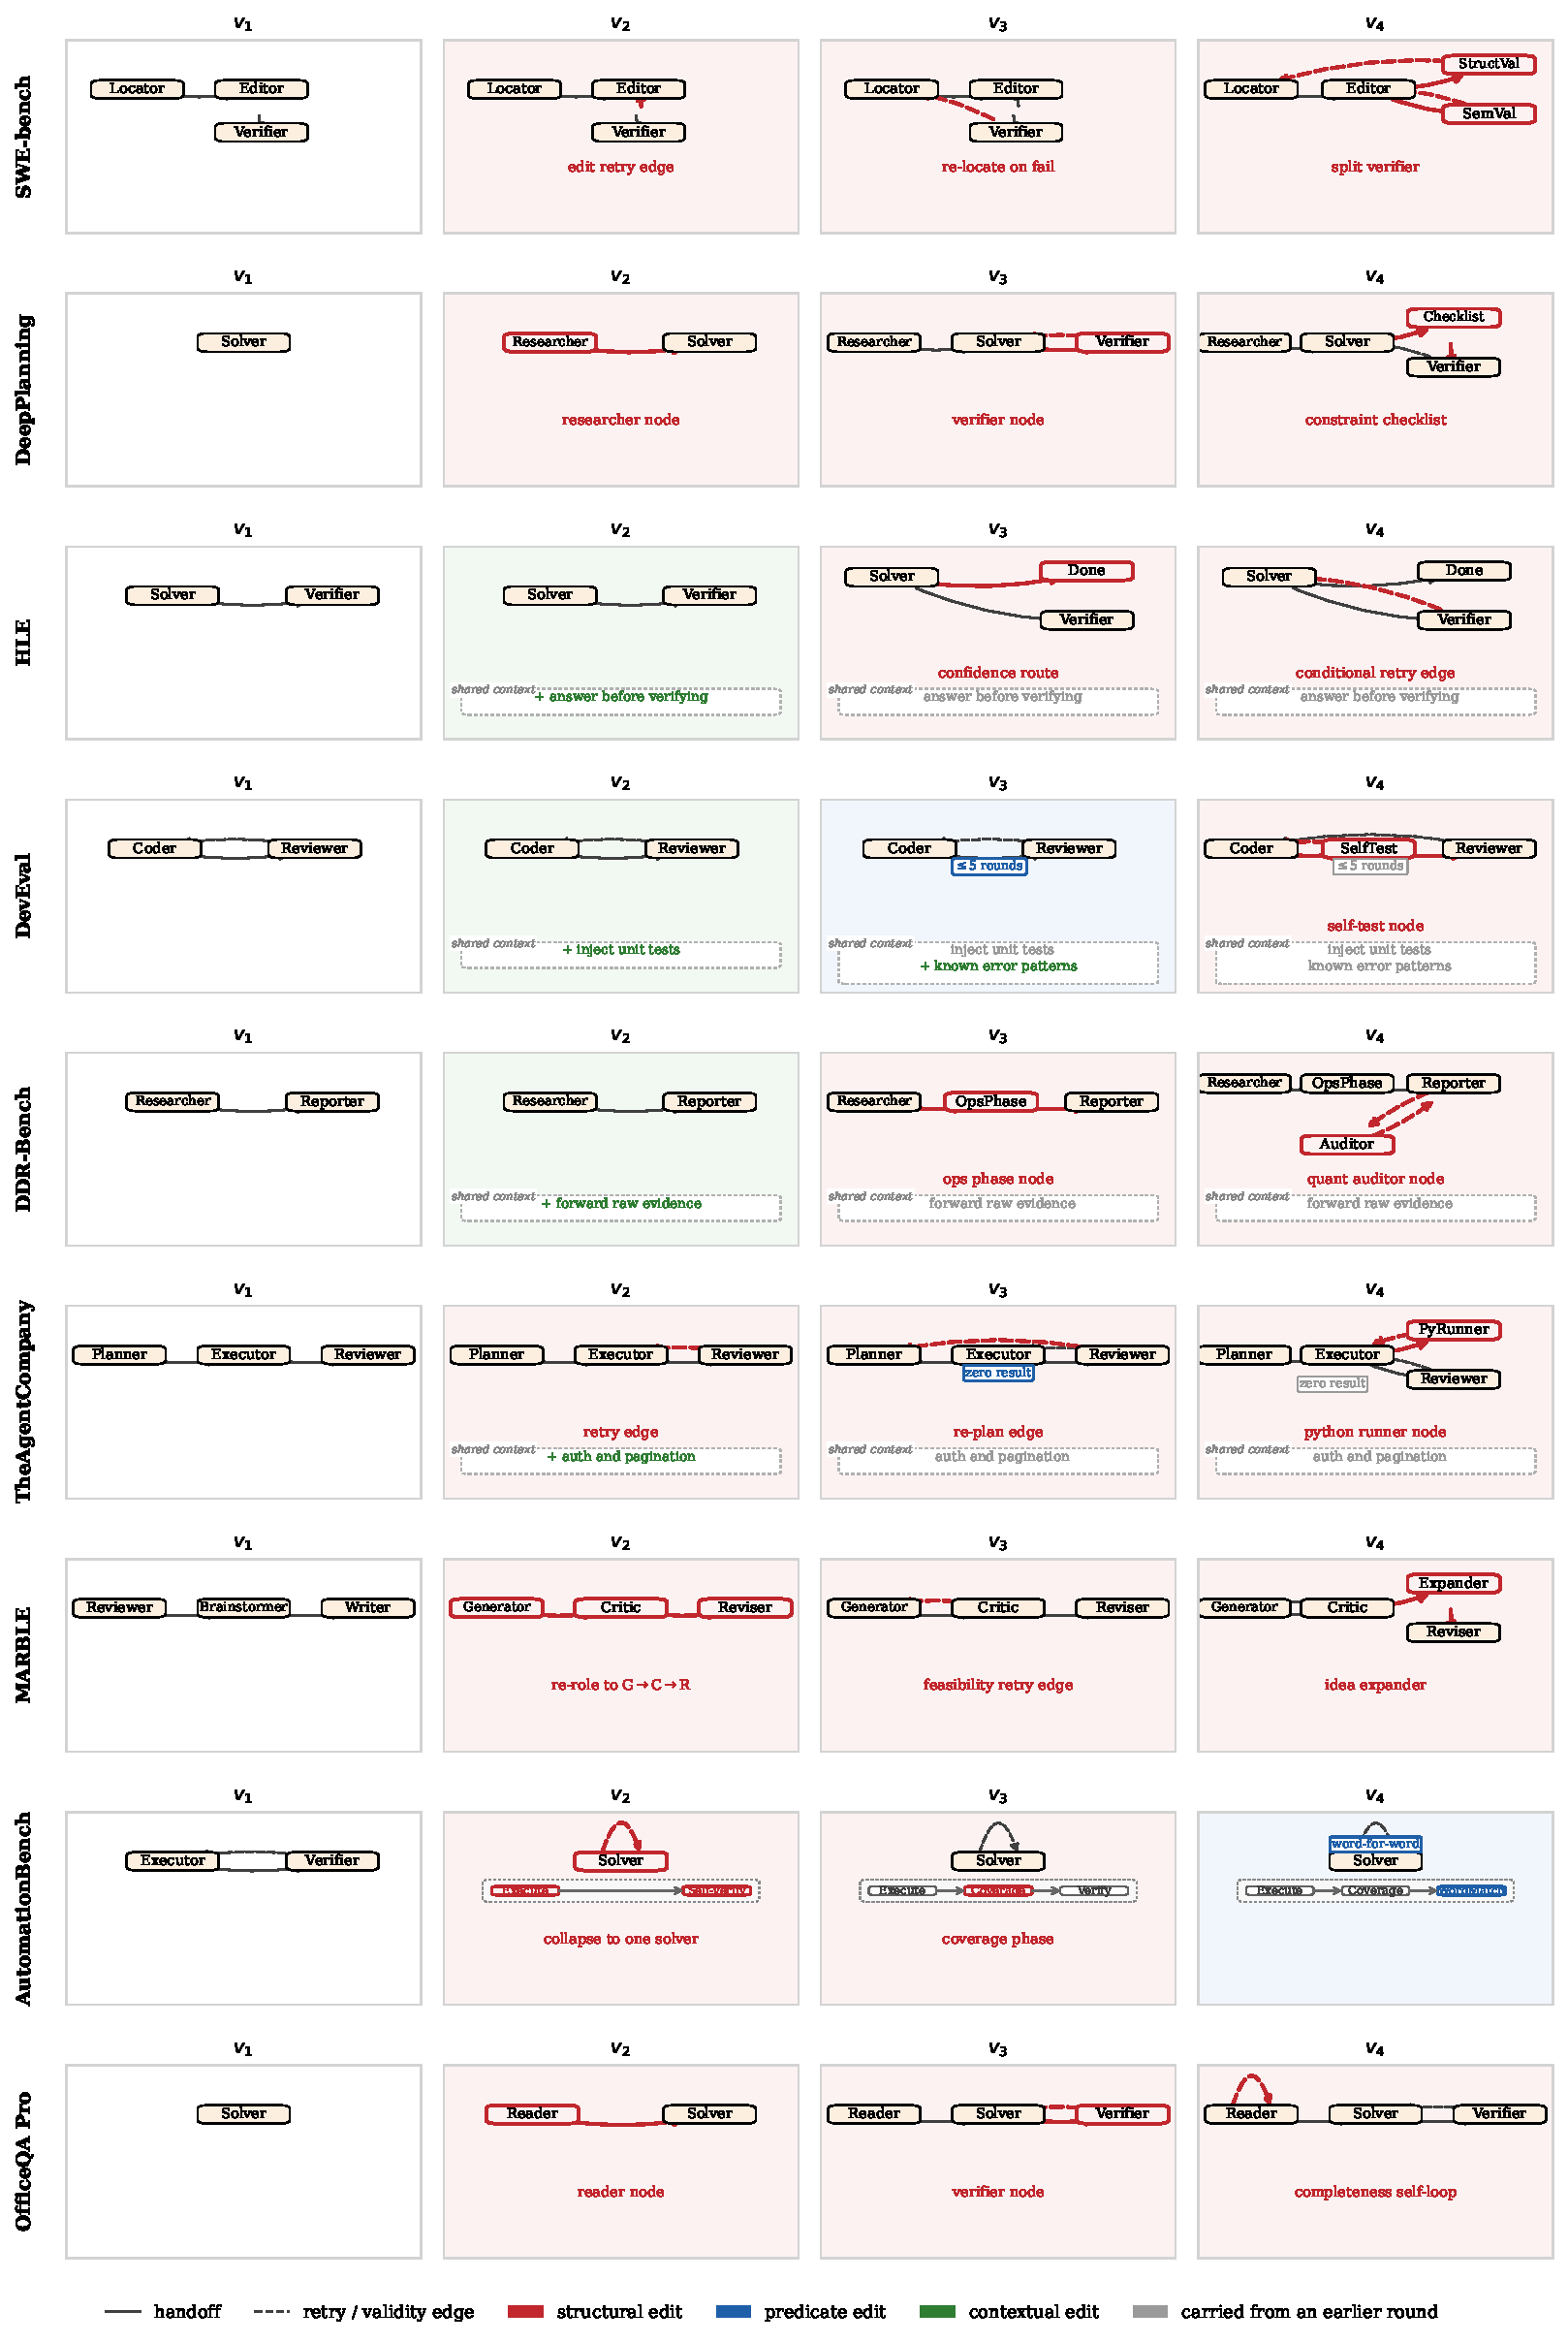
\includegraphics[width=0.97\linewidth]{figures/protocol_evolution.pdf}
\caption{Protocol evolution across rounds on the nine long-horizon and production-oriented benchmarks, one per row. Solid ovals are agent roles, pills inside a dashed container are internal phases of a single-agent solver, solid edges are admissible handoffs, and dashed edges are validity or retry edges. Boxed text pinned to an element is a transition or completion predicate, and the lower container holds the shared rule and culture. Elements introduced by the current round carry the color of their edit level from Section~\ref{sec:self_evolving} and earlier elements are gray, so a round that leaves the graph unchanged still shows what it revised.}
\label{fig:case_evo}
\end{figure}

\clearpage
\section{Per-benchmark Detailed Results}
\label{app:detail}

This appendix reports the per-benchmark results summarized in Table~\ref{tab:main}, and we also include the results of several other systems (taken from the leaderboard) as performance references. Table~\ref{tab:evolution_all} lists the primary metric of all fourteen benchmarks across the four evolution rounds. Tables~\ref{tab:humaneval}, \ref{tab:mbpp}, \ref{tab:gsm8k}, \ref{tab:math}, and \ref{tab:hotpot} detail the general question answering benchmarks, Tables~\ref{tab:swe}, \ref{tab:dp}, and \ref{tab:hle} the long-horizon benchmarks, and Tables~\ref{tab:deveval}, \ref{tab:ddr}, \ref{tab:tac}, \ref{tab:marble}, \ref{tab:autobench}, and \ref{tab:officeqa} the production-oriented benchmarks.

\begin{table}[t]
\caption{Primary metric across the four evolution rounds, each row in the benchmark's native metric.}
\label{tab:evolution_all}
\begin{center}
\small
\setlength{\tabcolsep}{3pt}
\begin{tabular}{lrrrrrr}
\toprule
\textbf{Benchmark} & \textbf{Single-agent} & \textbf{Multi-agent (init)} & $v_1$ & $v_2$ & $v_3$ & $v_4$ \\
\midrule
HumanEval & 87.5 & 96.9 & 98.4 & 100.0 & 100.0 & \textbf{100.0} \\
MBPP & 73.5 & 73.5 & 74.3 & 80.5 & 80.5 & \textbf{80.9} \\
GSM8K & 97.2 & 97.4 & 98.0 & 98.0 & 98.0 & \textbf{98.0} \\
MATH & 82.3 & 86.0 & 87.0 & 87.0 & 87.0 & \textbf{87.0} \\
HotpotQA & 75.9 & 64.0 & 80.7 & 81.9 & 82.3 & \textbf{82.3} \\
SWE-bench Verified & 75.6 & 67.0 & 78.8 & 85.6 & 85.8 & \textbf{86.2} \\
DeepPlanning & 45.0 & 33.8 & 44.6 & 44.6 & 54.2 & \textbf{54.2} \\
HLE (text-only) & 18.4 & 5.6 & 33.7 & 35.8 & 35.9 & \textbf{37.7} \\
DevEval & 62.5 & 82.1 & 82.1 & 83.9 & 90.6 & \textbf{96.9} \\
DDR-Bench & 42.8 & 44.0 & 44.0 & 58.9 & 66.5 & \textbf{76.0} \\
TheAgentCompany & 46.3 & 41.5 & 46.3 & 48.8 & 51.2 & \textbf{53.7} \\
MARBLE & 78.4 & 50.0 & 73.4 & 91.7 & 95.0 & \textbf{98.9} \\
AutomationBench & 23.7 & 23.6 & 26.1 & 28.4 & 34.8 & \textbf{54.8} \\
OfficeQA Pro & 35.3 & 21.1 & 31.6 & 62.4 & 67.7 & \textbf{69.9} \\
\bottomrule
\end{tabular}
\end{center}
\end{table}

\begin{table}[t]
\caption{Performance on HumanEval \citep{chen2021humaneval}. The metric is pass@1.}
\label{tab:humaneval}
\begin{center}\small
\begin{tabular}{lc}
\toprule
\textbf{Model / System} & \textbf{pass@1 (\%)} \\
\midrule
Direct LLM & 92.2 \\
\rowcolor{gray!12}
\textbf{OpenAgency} & \textbf{100.0} \\
\bottomrule
\end{tabular}\end{center}
\end{table}

\begin{table}[t]
\caption{Performance on MBPP \citep{austin2021mbpp}. The metric is pass@1.}
\label{tab:mbpp}
\begin{center}\small
\begin{tabular}{lc}
\toprule
\textbf{Model / System} & \textbf{pass@1 (\%)} \\
\midrule
Direct LLM & 69.3 \\
\rowcolor{gray!12}
\textbf{OpenAgency} & \textbf{80.9} \\
\bottomrule
\end{tabular}\end{center}
\end{table}

\begin{table}[t]
\caption{Performance on GSM8K \citep{cobbe2021gsm8k}. The metric is exact-match accuracy.}
\label{tab:gsm8k}
\begin{center}\small
\begin{tabular}{lc}
\toprule
\textbf{Model / System} & \textbf{Exact match (\%)} \\
\midrule
Direct LLM & 97.6 \\
\rowcolor{gray!12}
\textbf{OpenAgency} & \textbf{98.0} \\
\bottomrule
\end{tabular}\end{center}
\end{table}

\begin{table}[t]
\caption{Performance on MATH \citep{hendrycks2021math}. The metric is exact-match accuracy.}
\label{tab:math}
\begin{center}\small
\begin{tabular}{lc}
\toprule
\textbf{Model / System} & \textbf{Exact match (\%)} \\
\midrule
Direct LLM & 83.3 \\
\rowcolor{gray!12}
\textbf{OpenAgency} & \textbf{87.0} \\
\bottomrule
\end{tabular}\end{center}
\end{table}

\begin{table}[t]
\caption{Performance on HotpotQA \citep{yang2018hotpotqa}. The metric is token-level F1.}
\label{tab:hotpot}
\begin{center}\small
\begin{tabular}{lc}
\toprule
\textbf{Model / System} & \textbf{F1 (\%)} \\
\midrule
Direct LLM & 76.4 \\
\rowcolor{gray!12}
\textbf{OpenAgency} & \textbf{82.3} \\
\bottomrule
\end{tabular}\end{center}
\end{table}

\begin{table}[t]
\caption{Performance on SWE-bench Verified \citep{jimenez2024swebench}. FM is file match, and the first three rows are reported by that work.}
\label{tab:swe}
\begin{center}
\small
\begin{tabular}{lccc}
\toprule
\textbf{Model / System} & \textbf{\%Apply} & \textbf{FM} & \textbf{\%Resolved} \\
\midrule
Claude-2 & -- & -- & 4.8 \\
GPT-4 & -- & -- & 1.7 \\
SWE-Llama-13B & -- & -- & 3.9 \\
OpenHands                & 72.4 & 42.8 & 15.4 \\
\rowcolor{gray!12}
\textbf{OpenAgency} & \textbf{100.0} & \textbf{86.2} & \textbf{74.4} \\
\bottomrule
\end{tabular}
\end{center}
\end{table}

\begin{table}[t]
\caption{Performance on DeepPlanning \citep{zhang2026deepplanning}. Avg is the mean of travel and shopping case accuracy. External rows are reported by that work.}
\label{tab:dp}
\begin{center}
\small
\setlength{\tabcolsep}{2pt}
\begin{tabular}{lccccccc}
\toprule
\textbf{Model / System} & \textbf{Avg} & \textbf{Tra-CS} & \textbf{Tra-PS} & \textbf{Tra-Comp} & \textbf{Tra-Acc} & \textbf{Shop-M} & \textbf{Shop-Acc} \\
\midrule
Grok-4.1-Fast & 3.0 & 39.6 & 3.0 & 29.6 & 0.0 & 50.1 & 5.9 \\
GLM-4.7 & 7.1 & 38.9 & 7.1 & 30.7 & 0.0 & 61.2 & 14.2 \\
Qwen-Plus & 7.5 & 37.3 & 7.5 & 25.1 & 0.0 & 63.9 & 15.0 \\
Seed-1.8 & 11.3 & 43.0 & 11.3 & 45.3 & 0.0 & 68.1 & 22.5 \\
Kimi-K2-Thinking & 12.1 & 45.2 & 32.5 & 38.9 & 0.0 & 65.8 & 24.2 \\
DeepSeek-V3.2 & 21.6 & 47.4 & 35.0 & 41.2 & 0.7 & 78.8 & 42.5 \\
Gemini-3-Pro & 23.2 & 58.4 & 25.1 & 41.8 & 0.7 & 78.0 & 45.8 \\
o3 & 24.9 & 76.5 & 55.6 & 66.1 & 11.3 & 76.9 & 38.5 \\
Claude-Sonnet-4.5 & 25.5 & 65.2 & 58.4 & 61.8 & 7.6 & 80.0 & 43.3 \\
Qwen3-Max & 28.7 & 64.0 & 61.7 & 62.8 & 13.8 & 82.6 & 43.5 \\
Gemini-3-Flash & 28.8 & 67.1 & 57.7 & 62.4 & 5.9 & 80.6 & 51.7 \\
GPT-5 & 31.6 & 78.7 & 65.9 & 72.3 & 18.9 & 80.4 & 44.2 \\
Claude-Opus-4.5 & 33.9 & 79.3 & 70.9 & 75.1 & 22.7 & 80.0 & 45.0 \\
GPT-5.2 & 44.6 & 88.5 & 83.3 & 85.8 & 35.0 & 84.8 & 54.2 \\
\midrule
Qwen-Agent tool-calling & 46.9 & 88.8 & 56.7 & 72.7 & 32.9 & 86.8 & 60.8 \\
\rowcolor{gray!12}
\textbf{OpenAgency} & \textbf{54.2} & \textbf{90.1} & \textbf{85.6} & \textbf{87.3} & \textbf{38.4} & \textbf{87.5} & \textbf{62.1} \\
\bottomrule
\end{tabular}
\end{center}
\end{table}

\begin{table}[t]
\caption{Performance on the Humanity's Last Exam text-only subset. External rows are reported by the benchmark authors.}
\label{tab:hle}
\begin{center}
\small
\setlength{\tabcolsep}{6pt}
\begin{tabular}{lc}
\toprule
\textbf{Model / System} & \textbf{Accuracy (\%)} \\
\midrule
GPT-4o                          & 2.7 \\
Grok-2                          & 3.2 \\
Claude-Sonnet-3.5               & 4.3 \\
Gemini-1.5-Pro                  & 5.3 \\
Gemini-2.0-Flash-Thinking       & 8.1 \\
o1                              & 8.1 \\
o3-mini                          & 18.0 \\
\midrule
Direct LLM                                         & 13.4 \\
\rowcolor{gray!12}
\textbf{OpenAgency}                            & \textbf{37.7} \\
\bottomrule
\end{tabular}
\end{center}
\end{table}

\begin{table}[t]
\caption{Performance on DevEval \citep{li2024deveval}. UT is the unit-test pass rate and AT is the repository-level acceptance-test pass rate.}
\label{tab:deveval}
\begin{center}
\small
\setlength{\tabcolsep}{4pt}
\begin{tabular}{lcc}
\toprule
\textbf{Method} & \textbf{UT} & \textbf{AT} \\
\midrule
Direct LLM  & 90.4 & 62.5 \\
\rowcolor{gray!12}
\textbf{OpenAgency} & \textbf{99.1} & \textbf{96.9} \\
\bottomrule
\end{tabular}
\end{center}
\end{table}

\begin{table}[t]
\caption{Performance on the DDR-Bench 10-K subset \citep{liu2026ddrbench}. Overall averages Message-Wise and Trajectory-Wise accuracy. External rows are reported by that work.}
\label{tab:ddr}
\begin{center}
\small
\setlength{\tabcolsep}{7pt}
\begin{tabular}{lccc}
\toprule
\textbf{Model / System} & \textbf{Overall} & \textbf{Message-Wise} & \textbf{Trajectory-Wise} \\
\midrule
\multicolumn{4}{c}{\emph{Proprietary models}} \\
Gemini-2.5-Pro & 20.1 & 24.5 & 15.6 \\
Gemini-3-Flash & 33.0 & 44.8 & 21.2 \\
GPT-5.1 & 40.7 & 37.1 & 44.3 \\
GPT-5-mini & 42.0 & 46.8 & 37.1 \\
GPT-5.2 & 43.0 & 44.9 & 41.1 \\
Claude-Sonnet-4.5 & 69.1 & 77.6 & 60.6 \\
\midrule
\multicolumn{4}{c}{\emph{Open-source models}} \\
Llama-3.3-70B & 6.5 & 9.9 & 3.0 \\
Qwen2.5-72B & 20.3 & 27.1 & 13.4 \\
Qwen3-30B-A3B & 28.4 & 42.4 & 14.4 \\
MiniMax-M2 & 35.6 & 44.2 & 26.9 \\
Qwen3-Next-80B-A3B & 37.8 & 44.8 & 30.8 \\
Kimi-K2 & 41.0 & 51.1 & 30.8 \\
GLM-4.6 & 48.2 & 60.3 & 36.0 \\
DeepSeek-V3.2 & 49.2 & 60.1 & 38.2 \\
\midrule
DDR reference agent & 60.5 & 61.3 & 59.6 \\
\rowcolor{gray!12}
\textbf{OpenAgency} & \textbf{76.0} & 76.1 & \textbf{75.9} \\
\bottomrule
\end{tabular}
\end{center}
\end{table}

\begin{table}[t]
\caption{Performance on TheAgentCompany \citep{xu2024theagentcompany}. Score is the aggregated task score, and Steps is the average number of steps. External rows are reported by that work.}
\label{tab:tac}
\begin{center}
\small
\setlength{\tabcolsep}{5pt}
\begin{tabular}{llccc}
\toprule
\textbf{Model / System} & \textbf{Backbone} & \textbf{Success (\%)} & \textbf{Score (\%)} & \textbf{Steps ($\downarrow$)} \\
\midrule
OpenHands & Gemini-2.5-Pro & 30.3 & 39.1 & 33.5 \\
OpenHands & Claude-Sonnet-3.7 & 26.3 & 34.7 & 40.9 \\
OpenHands & Claude-Sonnet-3.5 & 24.0 & 34.4 & 29.2 \\
OpenHands & Gemini-2.0-Flash & 11.4 & 19.0 & 39.9 \\
OpenHands & GPT-4o & 8.6 & 16.7 & 28.7 \\
\midrule
OpenHands & GPT-5.5 & 40.0 & 41.5 & 31.6 \\
\rowcolor{gray!12}
\textbf{OpenAgency} & GPT-5.5 & \textbf{46.7} & \textbf{53.7} & \textbf{22.8} \\
\bottomrule
\end{tabular}
\end{center}
\end{table}

\begin{table}[t]
\caption{Performance on MARBLE \citep{zhu2025marble}. Overall averages Research and World scores. External rows are reported by that work.}
\label{tab:marble}
\begin{center}
\small
\setlength{\tabcolsep}{3pt}
\begin{tabular}{lcccc}
\toprule
\textbf{Model / System} & \textbf{Backbone} & \textbf{Research (\%)} & \textbf{World (\%)} & \textbf{Overall (\%)} \\
\midrule
Meta-Llama-3.1-8B      & Llama-3.1-8B  & 80.9 & 72.8 & 76.9 \\
Meta-Llama-3.1-70B     & Llama-3.1-70B & 80.8 & 72.1 & 76.5 \\
Meta-Llama-3.3-70B     & Llama-3.3-70B & 80.0 & 73.2 & 76.6 \\
GPT-3.5-turbo          & GPT-3.5-turbo & 70.2 & 71.7 & 71.0 \\
GPT-4o-mini & GPT-4o-mini   & 84.1 & 74.5 & 79.3 \\
\midrule
\rowcolor{gray!12}
\textbf{OpenAgency}                     & GPT-5.5       & \textbf{97.8} & \textbf{100.0} & \textbf{98.9} \\
\bottomrule
\end{tabular}
\end{center}
\end{table}

\begin{table}[t]
\caption{Performance on AutomationBench \citep{shepard2026automationbench}. External rows are reported by that work.}
\label{tab:autobench}
\begin{center}
\small
\setlength{\tabcolsep}{4pt}
\begin{tabular}{lc}
\toprule
\textbf{Model / System} & \textbf{Acc (\%)} \\
\midrule
GPT-6-Sol & 33.2 \\
GPT-6-Astra & 41.4 \\
Claude-Opus-5.5 & 42.5 \\
\midrule
\rowcolor{gray!12}
\textbf{OpenAgency} & \textbf{54.8} \\
\bottomrule
\end{tabular}
\end{center}
\end{table}

\begin{table}[t]
\caption{Performance on OfficeQA Pro \citep{opsahlong2026officeqa}. External rows are reported by that work.}
\label{tab:officeqa}
\begin{center}
\small
\setlength{\tabcolsep}{5pt}
\begin{tabular}{llc}
\toprule
\textbf{Model / System} & \textbf{Corpus format} & \textbf{Acc@1\% (\%)} \\
\midrule
GPT-5-mini                 & Full PDF                & 30.8 \\
GPT-5.4                    & Full PDF                & 36.1 \\
Gemini-3.1-Pro             & Full PDF                & 42.9 \\
GPT-5.1                    & Full PDF                & 45.1 \\
Claude-Opus-4.5            & Full PDF                & 46.6 \\
Claude-Opus-4.6 & ai\_parse\_document     & 57.1 \\
\midrule
Direct LLM                                               & Full PDF                & 26.3 \\
\rowcolor{gray!12}
\textbf{OpenAgency}                                  & Full PDF                & \textbf{69.9} \\
\bottomrule
\end{tabular}
\end{center}
\end{table}

\end{document}
